% ============================================================
%  CHAPITRE 4 — Section 4 : Augmentation par le pronostic (RB2(RUL))
% ============================================================

\section{Augmentation par le pronostic}
\label{sec:rul_aware}

% ------------------------------------------------------------
\subsection{Principe}
% ------------------------------------------------------------

La stratégie \RBsohH{} module l'effort en fonction de l'usure courante des composants. Deux composants partageant le même SoH ne sont cependant pas dans la même situation~: ce qui importe pour planifier l'effort à venir n'est pas seulement l'usure accumulée, mais le temps qui reste avant la fin de vie. C'est l'information portée par la durée de vie résiduelle (RUL).

La stratégie RB2(RUL) exploite ce pronostic plutôt que l'état présent. Dans le prolongement de \RBsohH, et pour les mêmes raisons liées aux mécanismes de dégradation dominants, seul l'offset de l'électrolyseur est dératé, en fonction de sa RUL estimée~: tant que la RUL reste élevée, l'électrolyseur assure un offset proche du nominal~; à l'approche de la fin de vie, l'offset est réduit pour étaler la dégradation restante et différer le remplacement.

% ------------------------------------------------------------
\subsection{Estimation de la RUL et formalisation}
% ------------------------------------------------------------

La durée de vie résiduelle est obtenue par extrapolation linéaire de la trajectoire de SoH jusqu'au seuil de fin de vie $\mathrm{SoH}_{\text{EoL}}$. Depuis le dernier remplacement, la pente moyenne de dégradation est estimée sur l'historique de SoH, et son intersection avec le seuil de fin de vie fournit le temps résiduel estimé, exprimé en jours. Cette estimation est rafraîchie à cadence hebdomadaire et n'est jugée fiable qu'au-delà d'un nombre minimal de points d'observation depuis le dernier remplacement~; tant que ce minimum n'est pas atteint, ou à l'état neuf, la RUL est ramenée à une valeur de référence par défaut, ce qui neutralise le levier.

Ce recours à une extrapolation linéaire mérite d'être souligné, car il s'écarte de la méthode de pronostic retenue au chapitre consacré au diagnostic et au pronostic. Ce dernier a privilégié un réseau récurrent LSTM, capable de capturer les tendances non linéaires et la courbure des trajectoires de dégradation, là où une extrapolation sécante les ignore. Le choix d'une simple extrapolation est ici délibéré et pragmatique~: rejouer l'inférence du réseau à chaque rafraîchissement hebdomadaire, sur un horizon de simulation de vingt-cinq ans, représenterait un coût de calcul prohibitif au regard de l'enjeu d'une étude comparative de stratégies. Il n'en demeure pas moins que la RUL alimentant RB2(RUL) est celle d'un substitut simplifié de la méthode de référence~: lorsque la dégradation s'accélère en fin de vie, l'extrapolation linéaire surestime la durée de vie résiduelle en négligeant la courbure descendante, et retarde d'autant l'activation du dérating~; à l'inverse, une pente localement pessimiste le déclencherait prématurément. L'apport propre du pronostic mesuré dans cette section est donc conditionné par la méthode d'extrapolation employée, et serait à réévaluer avec le réseau LSTM dans la boucle pour être pleinement représentatif.

Sur le modèle de \RBsohH, l'offset de l'électrolyseur est modulé par un facteur de dérating fonction de sa RUL estimée~:
\begin{equation}
\label{eq:rb2rul_offset}
P_{\text{ELY-offset}}(t) = f_{\text{ELY}}\!\big(\mathrm{RUL}_{\text{ELY}}(t)\big)\,P_{\text{ELY-offset}}^{0},
\qquad
f_{\text{ELY}}(\mathrm{RUL}) = \left[\,\min\!\left(\frac{\mathrm{RUL}_{\text{ELY}}}{\mathrm{RUL}^{\text{ref}}_{\text{ELY}}},\,1\right)\right]^{p_{\text{ELY}}},
\end{equation}
où $\mathrm{RUL}^{\text{ref}}_{\text{ELY}}$ est une durée de vie résiduelle de référence et $p_{\text{ELY}} \geq 0$ un exposant de modulation, analogue au $\gamma$ de \RBsohH. L'offset de la pile à combustible reste figé ($p_{\text{FC}} = 0$), pour la même raison qu'en \RBsohH~: sa dégradation, dominée par les démarrages-arrêts, n'est pas sensible au niveau d'offset.

L'estimateur en ligne a par ailleurs fait l'objet d'une vérification de non-régression. Un défaut d'ancrage — l'extrapolation prenait pour origine, après un remplacement, le SoH final de l'\emph{ancienne} unité au lieu de l'état neuf de la nouvelle — laissait la RUL figée à sa valeur par défaut pour toutes les unités suivant le premier remplacement, c'est-à-dire désactivait silencieusement le levier sur la fin de l'horizon. Ce défaut a été corrigé, couvert par un test de non-régression à usure artificiellement accélérée, et l'ensemble des résultats de cette section a été re-généré avec l'estimateur corrigé~; les écarts se sont avérés minimes (au plus $0{,}05$~k€ sur la grille de balayage), le levier n'agissant de toute façon qu'en fin de vie d'unité, période correctement simulée pour la première unité et où la seconde, jeune sur l'horizon restant, n'a presque rien à moduler. Les conclusions qui suivent sont donc établies avec un estimateur actif sur l'intégralité des vingt-cinq ans.

Le facteur $f_{\text{ELY}}$ est écrêté à $1$~: tant que la RUL estimée demeure supérieure à la référence $\mathrm{RUL}^{\text{ref}}_{\text{ELY}}$, aucun dérating n'est appliqué et RB2(RUL) coïncide exactement avec RB2, ce qui satisfait la propriété de test nul. Le levier ne s'active qu'à l'approche de la fin de vie, lorsque la RUL extrapolée chute sous la référence~: l'offset de l'électrolyseur est alors progressivement réduit pour ralentir sa dégradation restante et différer son remplacement. RB2(RUL) se distingue ainsi de \RBsohH~: là où \RBsohH{} module continûment l'effort dès les premiers signes d'usure, RB2(RUL) concentre l'allègement sur la phase terminale de vie, lorsque le pronostic annonce un remplacement imminent.

Les trois paramètres du levier — le socle $P_{\text{ELY-offset}}^{0}$, la référence $\mathrm{RUL}^{\text{ref}}_{\text{ELY}}$ et l'exposant $p_{\text{ELY}}$ — ont été calés par balayage conjoint sur l'horizon de vingt-cinq ans, en minimisant le coût total unifié (VoLL~$=3$~€/kWh). Ce balayage conjoint est essentiel pour une comparaison honnête~: c'est en balayant \emph{aussi} le socle $P_{\text{ELY-offset}}^{0}$ que l'on compare le meilleur RB2(RUL) au meilleur RB2 (comparaison « best-vs-best »), et non à un RB2 nominal non optimisé qui surestimerait artificiellement l'apport du pronostic. La grille couvre le socle ($c_{\text{ELY}} \in \{0{,}300\,;0{,}310\,;0{,}320\}$), l'exposant ($p_{\text{ELY}} \in \{0\,;0{,}05\,;0{,}10\,;0{,}20\,;0{,}50\}$) et le seuil ($\mathrm{RUL}^{\text{ref}}_{\text{ELY}} \in \{1000\,;2000\,;3000\}$~jours), le socle de la pile à combustible restant fixé à son meilleur RB2 ($c_{\text{FC}} = 0{,}440$). L'enseignement de ce balayage, développé à la sous-section suivante, est que l'exposant optimal est nul.

% ------------------------------------------------------------
\subsection{Résultats}
% ------------------------------------------------------------

Le balayage conjoint décrit ci-dessus livre un résultat sans ambiguïté~: l'exposant de dérating qui minimise le coût total unifié est \emph{nul}. Le Tableau~\ref{tab:rb2rul_sweep} en donne un extrait à socle et seuil fixés à leur meilleure valeur ($c_{\text{ELY}} = 0{,}310$, $\mathrm{RUL}^{\text{ref}}_{\text{ELY}} = 1000$~jours), en faisant croître le seul exposant.

\begin{table}[h!]
\centering
\caption{Effet de l'exposant de dérating RUL sur les indicateurs (balayage à socle et seuil optimaux, $c_{\text{ELY}} = 0{,}310$, $\mathrm{RUL}^{\text{ref}} = 1000$~j, VoLL~$=3$~€/kWh). L'exposant nul, c'est-à-dire l'absence de modulation, minimise le coût total~: toute modulation croissante dégrade le compromis.}
\label{tab:rb2rul_sweep}
\begin{tabular}{cccc}
\hline
$p_{\text{ELY}}$ & LPSP [\%] & Coût de dégradation [k€] & Coût total [k€] \\
\hline
$0$ (= RB2)     & 2,592 & 58,84 & \textbf{80,10} \\
$0{,}05$        & 2,609 & 58,71 & 80,10 \\
$0{,}10$        & 2,711 & 58,50 & 80,74 \\
$0{,}20$        & 2,852 & 58,25 & 81,65 \\
$0{,}50$        & 3,143 & 58,05 & 83,82 \\
\hline
\end{tabular}
\end{table}

La lecture est nette. Augmenter l'exposant abaisse bien légèrement le coût de dégradation, de $58{,}85$ à $58{,}05$~k€, en bridant davantage l'électrolyseur en fin de vie~; mais cet allègement se paie par une hausse plus que proportionnelle de la LPSP, de $2{,}59$ à $3{,}14\,\%$, si bien que le coût total unifié \emph{croît} continûment, de $80{,}11$ à $83{,}83$~k€. Le meilleur point modulé ($p_{\text{ELY}} = 0{,}05$) affiche un coût total de $80{,}104$~k€, à comparer aux $80{,}102$~k€ du cas non modulé~: l'écart apporté par le levier RUL est de $+0{,}002$~k€, soit $0{,}002\,\%$, autant dire nul. À socle optimisé, la modulation par le pronostic n'améliore donc pas la stratégie de référence~: le levier RB2(RUL) retombe sur RB2.

Ce résultat corrige une conclusion trop optimiste qu'aurait donnée une comparaison biaisée. Rapporté à un RB2 nominal non optimisé, le dérating RUL semblait apporter un gain de durabilité~; mais ce gain provenait en réalité de l'abaissement du socle de l'électrolyseur, et non du pronostic. Une fois le socle de RB2 lui-même optimisé — ce qui conduit exactement aux réglages de RB2(RUL) à exposant nul —, l'apport propre du pronostic s'évanouit. Le Tableau~\ref{tab:rb2rul_results} résume les points retenus~: RB2(RUL) est confondu avec RB2, tandis que \RBsohH, qui module sur l'état de santé, conserve, lui, un gain réel.

\begin{table}[h!]
\centering
\caption{Points de fonctionnement retenus (best-vs-best, coût total unifié à VoLL~$=3$~€/kWh). RB2(RUL) coïncide avec RB2~; seule la modulation par le SoH apporte un gain.}
\label{tab:rb2rul_results}
\begin{tabular}{lccc}
\hline
Stratégie & LPSP [\%] & Coût de dégradation [k€] & Coût total [k€] \\
\hline
RB2 (référence) & 2,59 & 58,85 & 80,11 \\
RB2(RUL)        & 2,59 & 58,85 & 80,11 \\
\RBsohH{}       & 2,91 & 54,91 & 78,77 \\
\hline
\end{tabular}
\end{table}

Le positionnement dans le plan de Pareto est reporté à la Figure~\ref{fig:pareto_rb2rul}. RB2(RUL) se superpose exactement à RB2 (point figuré par un anneau creux autour de RB2), tandis que \RBsohH{} se détache sur une droite d'iso-coût unifié plus basse.

\begin{figure}[h!]
    \centering
    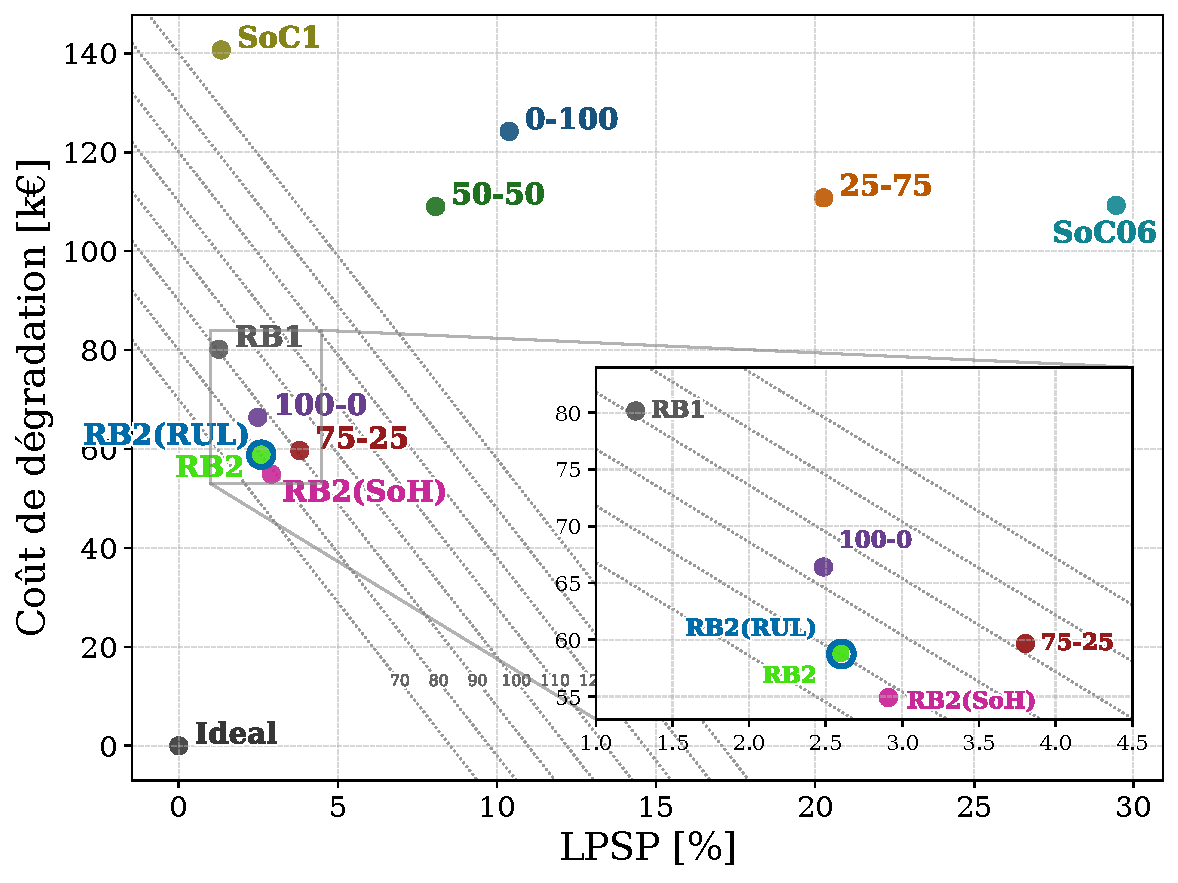
\includegraphics[width=\linewidth]{Chapitre 3/RUL/Figures/pareto_rul_isocost.pdf}
    \caption{Positionnement de RB2(RUL) dans le plan de Pareto LPSP--coût de dégradation, avec RB2 et \RBsohH, parmi le panel du chapitre précédent (agrandissement sur l'amas RB2 en encart). RB2(RUL) à son optimum (exposant nul) se confond avec RB2~: il est figuré par un anneau creux superposé au point RB2. Les droites pointillées grises sont les lignes d'iso-coût total unifié (dégradation $+$ valorisation de la LPSP à VoLL~$=3$~€/kWh, pente $8{,}2$~k€ par point de LPSP)~; leur étiquette donne le coût total en k€.}
    \label{fig:pareto_rb2rul}
\end{figure}
\FloatBarrier

Cette absence d'apport du pronostic mérite d'être commentée, car elle tient à deux raisons complémentaires.

La première raison est que la RUL n'apporte, sur ce cas d'étude, aucune information \emph{intrinsèque} supplémentaire par rapport au seul état de santé. \RBsohH{} et RB2(RUL) exploitent \emph{in fine} la même grandeur physique, l'usure de l'électrolyseur, l'une par son niveau courant (SoH), l'autre par sa projection (RUL). Or la RUL n'est ici qu'une transformation déterministe du SoH, obtenue en extrapolant sa trajectoire jusqu'au seuil de fin de vie~: elle ne contient rien que le SoH, et sa pente, ne portent déjà. Moduler sur la RUL plutôt que sur le SoH ne fait donc qu'exploiter, de manière détournée, la même information — et une fois le socle optimisé, cette modulation supplémentaire n'a plus de marge à récupérer.

La seconde raison est que la RUL est \emph{peu fiable}, tout particulièrement là où le levier voudrait agir. Estimer une durée de vie résiduelle suppose d'extrapoler une tendance de dégradation~; or, en début de vie d'un composant, cette tendance est mal établie — peu de points d'historique, dégradation encore lente qui n'a pas révélé son éventuelle accélération future — et l'extrapolation est très imprécise. Le seuil de dérating ($\mathrm{RUL} < \mathrm{RUL}^{\text{ref}}$) peut alors être franchi ou non au gré du bruit d'estimation, si bien que les modulations de puissance déclenchées par la RUL sont, sur une large part de la vie du composant, essentiellement \emph{aléatoires}. Une commande pilotée par un signal aussi bruité ne peut structurellement pas améliorer le compromis~: au mieux elle n'y touche pas, au pire elle bride l'électrolyseur au mauvais moment. C'est cohérent avec le résultat du balayage, qui préfère ne pas moduler du tout.

Ce constat resterait à nuancer dans un contexte où la dégradation s'accélère nettement et \emph{régulièrement} en fin de vie~: la projection de la RUL y anticiperait un franchissement de seuil que le SoH instantané ne signale pas encore, et le pronostic reprendrait alors un avantage — à condition que cette accélération soit assez régulière pour être extrapolée avec une incertitude maîtrisée, ce qui n'est pas le cas ici.

% ------------------------------------------------------------
\subsection{Sensibilité à l'incertitude du pronostic}
\label{subsec:rb2rul_uncertainty}
% ------------------------------------------------------------

Les résultats précédents supposent une RUL parfaitement connue. Or le pronostic est, par nature, entaché d'incertitude, et c'est ici que la distinction entre diagnostic et pronostic prend tout son sens. Le chapitre consacré au pronostic a quantifié cette incertitude par Monte-Carlo \textit{dropout}~: chaque prédiction de SoH est assortie d'un intervalle de confiance empirique à $95\,\%$, dont la largeur croît avec l'horizon de projection. La RUL étant l'abscisse de l'intersection entre la trajectoire de SoH projetée et le seuil de fin de vie, elle \emph{amplifie} cette incertitude~: une faible dispersion sur la pente ou le niveau du SoH se traduit par une dispersion bien plus large sur le temps d'atteinte du seuil. Les bornes optimiste et conservatrice de la RUL de l'électrolyseur, obtenues au chapitre dédié à partir des percentiles des trajectoires prédites, encadrent ainsi une plage d'autant plus étendue que l'horizon visé est lointain.

Cette amplification a une conséquence directe sur les deux stratégies. \RBsohH{} fonde sa décision sur l'\emph{état de santé instantané}, dont l'incertitude est celle du seul diagnostic~; une décision fondée sur la RUL porte, elle, l'incertitude du diagnostic \emph{propagée et amplifiée} par l'extrapolation jusqu'au seuil de fin de vie. C'est la traduction quantitative de la seconde raison invoquée plus haut~: le signal qui pilote la modulation RUL est bien plus bruité que le SoH, ce qui rend cette modulation peu fiable.

Pour l'objectiver, on propage l'incertitude mesurée du pronostic ($\sigma_{\mathrm{RUL}}/\mathrm{RUL}$ dépendant de l'horizon, quantifié au chapitre dédié) par Monte-Carlo sur les points de fonctionnement, en considérant une variante \emph{modulée} de RB2(RUL) (exposant non nul) — puisque le point retenu, non modulé, est insensible par construction à la RUL. Le résultat est reporté à la Figure~\ref{fig:rb2rul_ellipses}~: l'ellipse d'incertitude $1\sigma/2\sigma$ de RB2(RUL) est sensiblement plus étendue que le point quasi ponctuel de \RBsohH. Autrement dit, dès qu'on module sur la RUL, l'incertitude du pronostic disperse le point de fonctionnement sans le déplacer en moyenne vers un meilleur compromis~: la modulation ajoute du bruit, pas de la performance. Ce constat rejoint celui du balayage, qui préfère l'absence de modulation.

\begin{figure}[h!]
    \centering
    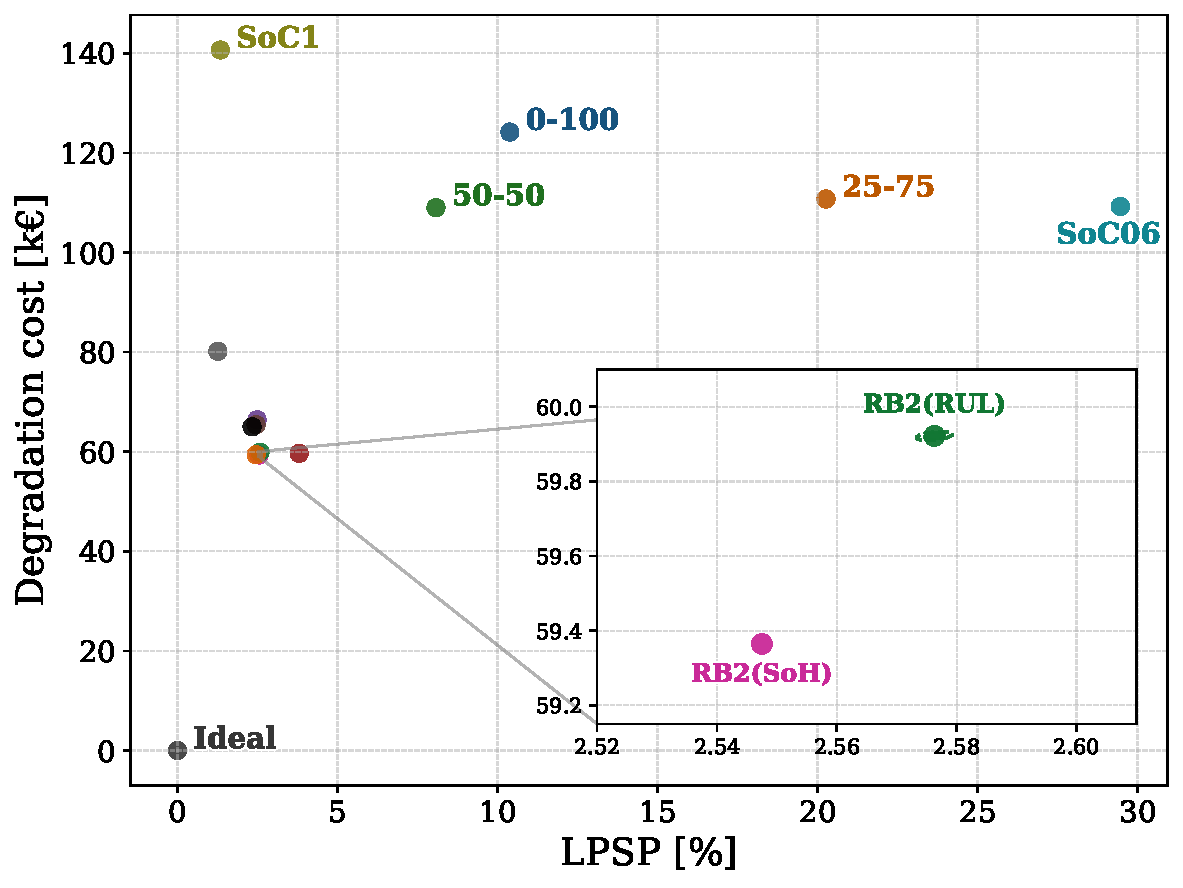
\includegraphics[width=\linewidth]{Chapitre 3/RUL/Figures/rb2rul_ellipses.pdf}
    \caption{Dispersion du point de Pareto de RB2(RUL) sous propagation de l'incertitude du pronostic (ellipses $1\sigma/2\sigma$ recentrées sur le point nominal, Monte-Carlo), face au point de \RBsohH. Le panel complet situe l'amas RB2 dans le plan de Pareto (encart).}
    \label{fig:rb2rul_ellipses}
\end{figure}
\FloatBarrier

Quantitativement (Monte-Carlo à \num{200} tirages, incertitude relative $\sigma_{\mathrm{RUL}}/\mathrm{RUL}$ dépendant de l'horizon interpolée sur la courbe mesurée au chapitre dédié, rafraîchissement hebdomadaire), le demi-grand axe à $1\sigma$ de l'ellipse de RB2(RUL) modulé vaut environ quatre fois celui de \RBsohH{} ($6{,}0\times 10^{-3}$ contre $1{,}5\times 10^{-3}$ dans les unités du plan). Les deux dispersions restent faibles dans l'absolu — l'agrégation sur vingt-cinq ans moyenne l'essentiel du bruit d'estimation, et le levier RUL s'active tard dans la vie de l'électrolyseur, précisément là où l'incertitude relative de la RUL passe par son minimum ($\approx 5\,\%$ vers 400--450~jours d'horizon) — mais le rapport d'un facteur quatre entre les deux signaux illustre le coût, en dispersion, de la décision fondée sur une grandeur extrapolée plutôt qu'instantanée.

Au total, pour le présent cas d'étude, l'augmentation par le pronostic n'apporte rien de plus que l'augmentation par le diagnostic~: à socle optimisé, RB2(RUL) retombe sur RB2, tandis que \RBsohH{} — qui exploite \emph{in fine} la même usure de l'électrolyseur, mais à partir d'un signal instantané mieux maîtrisé — conserve seul un gain réel. La connaissance supplémentaire que porterait la RUL, à savoir le \emph{rythme} d'usure projeté, est ici à la fois redondante avec le SoH et trop incertaine, en particulier en début de vie, pour être exploitée de manière fiable. Le pronostic ne reprendrait l'avantage que dans un contexte où la dégradation s'accélère nettement et régulièrement en fin de vie — situation où la projection anticiperait un franchissement de seuil que le SoH instantané ne contient pas encore, et où cette accélération serait assez régulière pour être pronostiquée avec une incertitude maîtrisée.
